\documentclass[10pt,a4paper]{article}
\usepackage[utf8]{inputenc}
\usepackage[T1]{fontenc}
\usepackage{lmodern}
\usepackage[margin=1.5cm, top=1.4cm, bottom=1.4cm]{geometry}
\usepackage{hyperref}
\usepackage{enumitem}
\usepackage{titlesec}
\usepackage{xcolor}
\usepackage{graphicx}

\definecolor{accent}{HTML}{00686E}
\hypersetup{colorlinks=true, urlcolor=accent, linkcolor=accent}
\pagenumbering{arabic}
\setlength{\parindent}{0pt}

\titleformat{\section}{\large\bfseries\color{accent}}{}{0em}{}[\vspace{-0.6em}\rule{\textwidth}{0.8pt}]
\titlespacing{\section}{0pt}{7pt}{4pt}

\newcommand{\role}[4]{%
  \textbf{#1} \hfill \textbf{#2}\\[1pt]%
  \textit{#3} \hfill \textit{#4}\\[2pt]%
}
\setlist[itemize]{leftmargin=1.2em, itemsep=1.5pt, topsep=2pt, parsep=0pt}

\begin{document}

% ================= HEADER =================
\begin{minipage}[c]{0.80\textwidth}
  {\Huge\bfseries Prabhavit Gupta}\\[3pt]
  {\color{accent}\large Generative AI \& LLM Engineer: Agent Architectures, RAG \& Python}\\[6pt]
  {\footnotesize +39 351 610 7807 ~$\vert$~
  \href{mailto:prabhavitg@gmail.com}{prabhavitg@gmail.com} ~$\vert$~
  \href{https://www.linkedin.com/in/prabhavit/}{linkedin.com/in/prabhavit} ~$\vert$~
  \href{https://github.com/prab-gupta}{github.com/prab-gupta} ~$\vert$~
  Venice, Italy (CET Time Zone / EU Permanent Resident / Available Immediately)}
\end{minipage}\hfill
\begin{minipage}[c]{0.18\textwidth}
  \raggedleft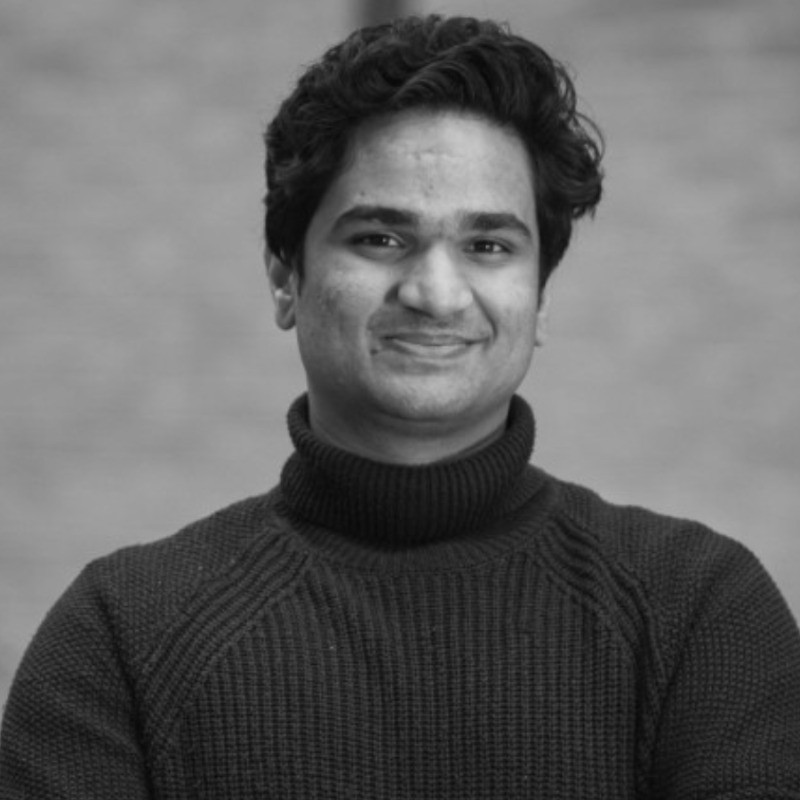
\includegraphics[width=2.0cm]{photo.jpg}
\end{minipage}
\vspace{-2pt}

% ================= SUMMARY =================
\section{Summary}
Generative AI and Large Language Model (LLM) Systems Engineer with 3 years of commercial production experience designing, deploying, and optimizing enterprise agentic systems, RAG pipelines, and high-throughput Python backends. Extensive hands-on experience building production workflows powered by frontier models (Claude, GPT-4, Llama 3) using LangChain, LlamaIndex, and Model Context Protocol (MCP). Proven track record implementing semantic caching, token optimization, prompt engineering, and automated LLM evaluation harnesses that reduce inference latency and API costs. Dedicated, results-driven engineer available immediately for full-time remote roles without notice period.

% ================= TECHNICAL EXPERTISE =================
\section{Technical Expertise}
\begin{itemize}
  \item \textbf{Generative AI \& LLMs:} Claude 3.5 Sonnet, GPT-4o, Llama 3, Mistral, LangChain, LlamaIndex, Model Context Protocol (MCP), tool-calling agents, few-shot prompting, system prompt design.
  \item \textbf{RAG \& Vector Architecture:} Vector indexing (Chroma, PGVector, FAISS), hybrid search, semantic chunking, embedding fine-tuning, metadata filtering, semantic caching with Redis.
  \item \textbf{Backend \& Microservices:} Python (FastAPI, asyncio, Pydantic, requests), RESTful APIs, asynchronous worker queues (Celery, Redis), schema validation, rate-limiting, and error recovery.
  \item \textbf{Evaluation \& Optimization:} Automated evaluation harnesses (RAGAS, prompt regression suites), token reduction strategies, context window management, cost/latency profiling.
  \item \textbf{Cloud \& DevOps:} Docker containerization, Kubernetes orchestration, GitHub Actions CI/CD workflows, Linux server management, structured telemetry logging.
  \item \textbf{Languages \& Availability:} English (C1 Professional, fluent), Hindi (Native), Italian (Conversational). Available immediately without notice period.
\end{itemize}

% ================= EXPERIENCE =================
\section{Experience}

\role{\href{https://flowspace.co}{FlowSpace.co}}{Mar 2024 - Aug 2026}{Lead Generative AI \& Agent Architect}{London, UK (remote)}
\begin{itemize}
  \item Architected and deployed multi-agent production workflows in Python and FastAPI, leveraging Claude 3.5 Sonnet and GPT-4 to automate enterprise knowledge extraction for 4,500+ users.
  \item Built advanced RAG pipelines featuring semantic chunking, dense vector retrieval, and reranking, improving retrieval precision by 34\% across complex technical documentation.
  \item Implemented semantic response caching with Redis and token compression strategies, reducing third-party LLM API inference costs by 38\% while maintaining high fidelity.
  \item Developed automated evaluation harnesses running prompt regression tests on GitHub Actions CI/CD to prevent drift and hallucination across model updates.
  \item Integrated custom Model Context Protocol (MCP) servers allowing agents to safely invoke analytical database queries and external CRM actions.
\end{itemize}

\role{Urlink}{Apr 2025 - Jul 2025}{AI Platform Developer (Freelance)}{Barcelona, Spain (remote)}
\begin{itemize}
  \item Developed custom LLM data extraction microservices in Python, parsing semi-structured web feeds and generating standardized JSON schemas via Pydantic.
  \item Containerized AI microservices using Docker and integrated them with message brokers and asynchronous queues for batch processing.
  \item Implemented automated integration tests with pytest and Playwright to validate end-to-end LLM application workflows and latency constraints.
\end{itemize}

\role{Independent Technical Consultant}{Aug 2023 - Feb 2024}{Applied AI \& Python Developer}{Venice, Italy}
\begin{itemize}
  \item Engineered custom Generative AI assistants and document summarization bots for European SMB clients using LangChain and OpenAI APIs.
  \item Built automated ETL scripts in Python ingesting local documents into vectorized knowledge bases with SQLite and ChromaDB.
  \item Authored technical architecture runbooks and prompt engineering guidelines for client engineering teams.
\end{itemize}

% ================= EDUCATION =================
\section{Education}
\role{Ca' Foscari University of Venice}{2020 - 2024}{BA in Philosophy, International Studies and Economics}{Venice, Italy}
\begin{itemize}
  \item Rigorous training in formal logic, statistical inference, quantitative economics, and complex systems modeling.
\end{itemize}

\end{document}
